\documentclass[tikz, border=3.14mm]{standalone}
\usepackage{circuitikz}

\begin{document}
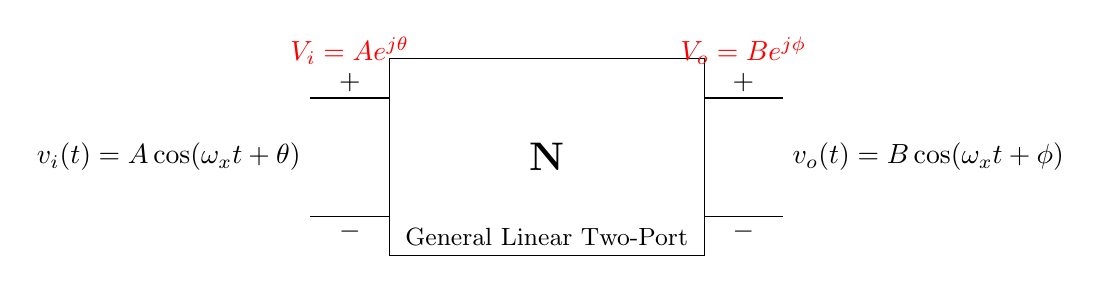
\begin{tikzpicture}[american]
    % Draw the two-port network box
    \draw (0,0) rectangle (4,2.5);
    \node at (2,1.25) {\Large \textbf{N}};
    \node[anchor=south] at (2,0) {\small General Linear Two-Port};
    
    % Input side
    \draw (-1,2) -- (0,2);
    \draw (-1,0.5) -- (0,0.5);
    \node[anchor=east] at (-1,1.25) {$v_i(t) = A \cos(\omega_x t + \theta)$};
    \node at (-0.5, 2.2) {$+$};
    \node at (-0.5, 0.3) {$-$};
    
    % Output side
    \draw (4,2) -- (5,2);
    \draw (4,0.5) -- (5,0.5);
    \node[anchor=west] at (5,1.25) {$v_o(t) = B \cos(\omega_x t + \phi)$};
    \node at (4.5, 2.2) {$+$};
    \node at (4.5, 0.3) {$-$};
    
    % Phasor labels
    \node[red] at (-0.5, 2.6) {$V_i = A e^{j\theta}$};
    \node[red] at (4.5, 2.6) {$V_o = B e^{j\phi}$};

\end{tikzpicture}
\end{document}
